\section{Background}\label{sec:background}
\label{sec:cast}

In this section, we define the terms needed to state Gauss-Bonnet theorem.
We then present two proofs one for a continuous version and one for a discrete version.


\subsection{Curvature}

The Gauss-Bonnet theorem relates local curvature calculations
to global topology. 
We will see several definitions of curvature.
Some definitions lend themselves to computations and others provide
more geometric intuition.
Intuitively, a straight line should have zero curvature and
 large circles should have smaller curvature than smaller circles.
 We would also like to differentiate
curving to the left and curving to the right..

In one dimension, for any point on a curve
we can approximate the curve with a circle.
The best approximating circle is the  \EMPH{osculating circle}.
 We can define the \EMPH{curvature} to be the inverse of the radius of this circle $k=\frac{1}{r}$.
See \figref{osculating-circle} for an example.
In the plane, we determine the sign by which side of the curve the osculating circle is on.
 This osculating-circle idea can be extend
to  surfaces in $\R^3$, by considering the \EMPH{osculating sphere},
But notice that at saddle points on a surface it is not clear which sphere
best approximates the surface.
The above definition provides great intuition for the curvature of curves
and surfaces but in many applications we would like a formula to compute
the curvature of a curve or surface.


\begin{figure}[htb]
	\centering
	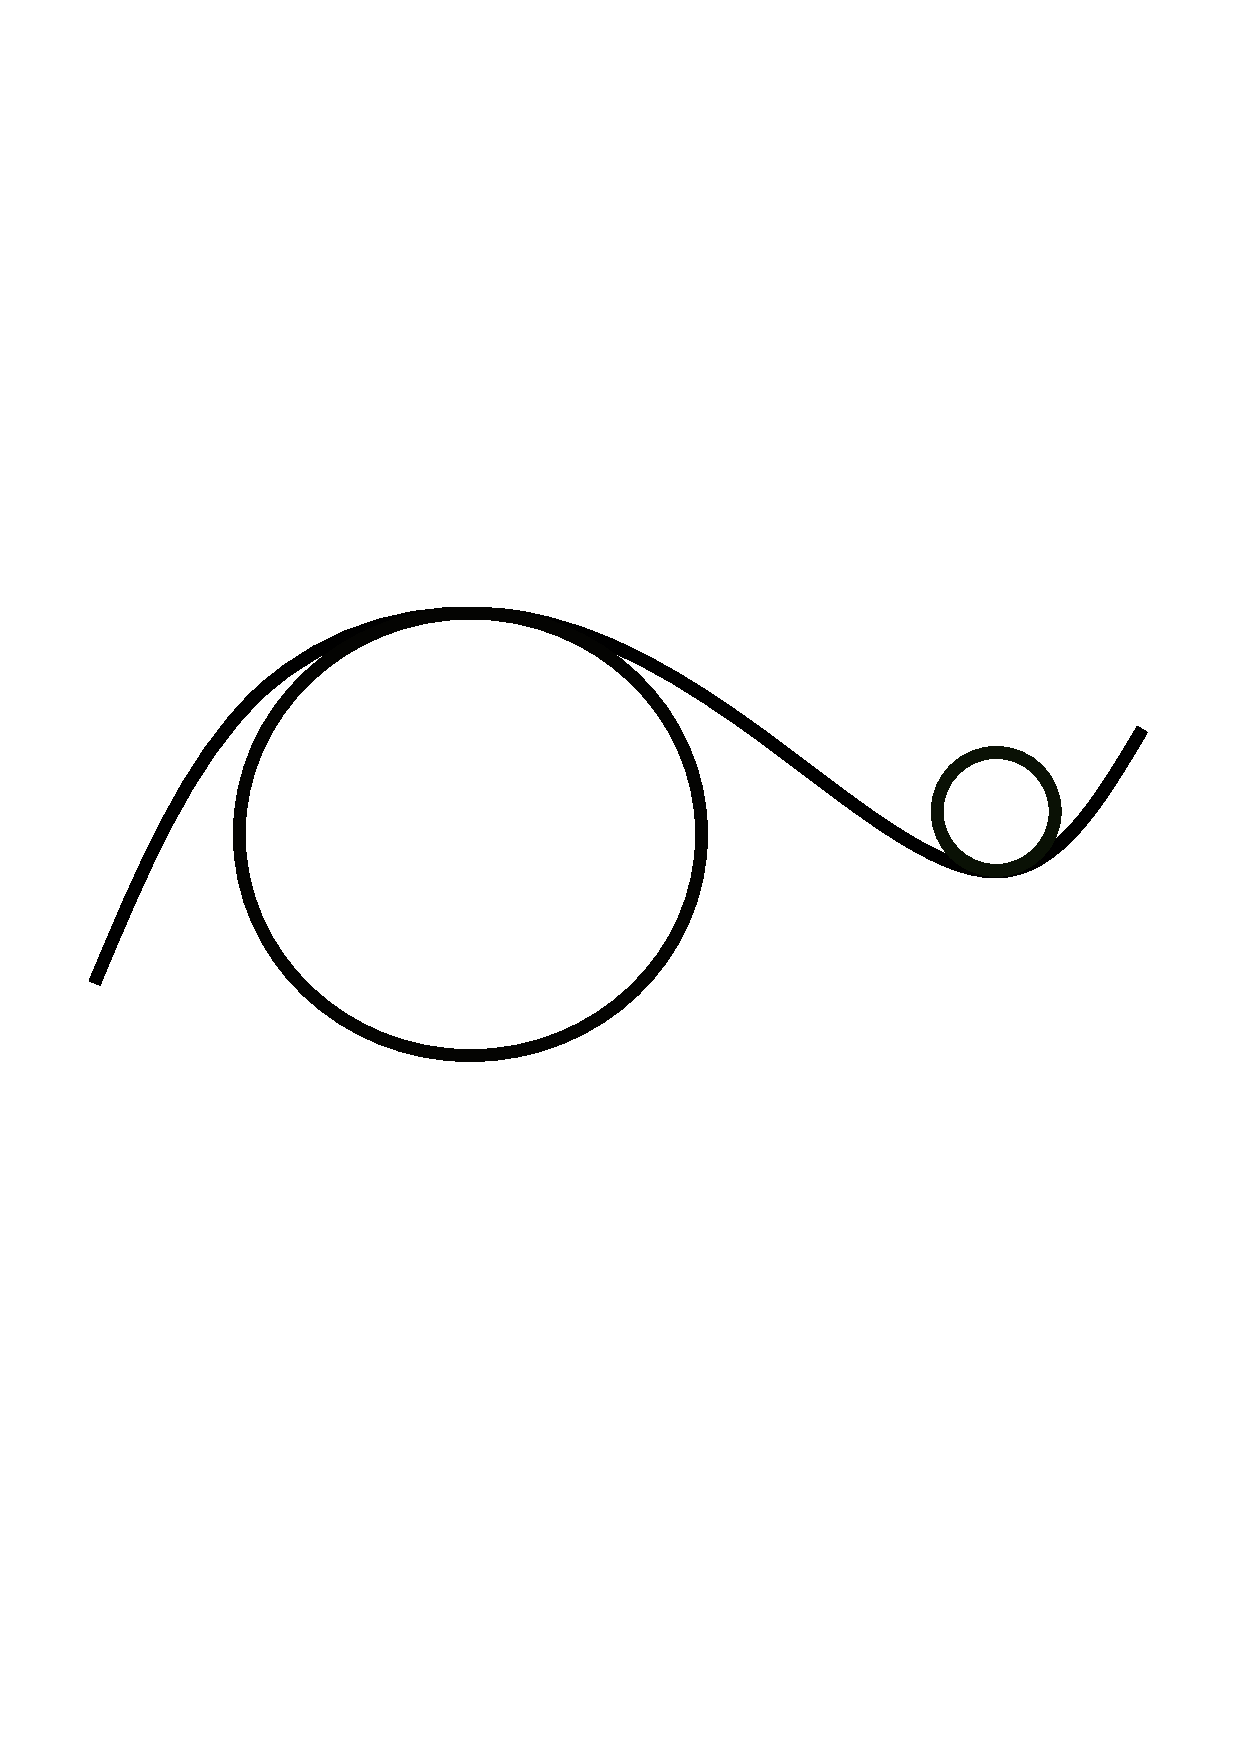
\includegraphics[width=.3\textwidth]{curvature/osculating}
	\caption{A curve with two osculating circles. The curvature at these points
	have opposite sign.}
	\label{fig:osculating-circle}
\end{figure}

A curve in $\RR^3$ is often presented as a function
$\gamma(t)=(x(t),y(t),z(t))$ that  is \EMPH{smooth} on an open interval $I$
if $\gamma'$ is continuous and $\gamma'(t)\neq (0,0,0)$ on $I$. 
If $\gamma$ is smooth it has a well-defined unit tangent vector $T(t)=\frac{\gamma'(t)}{|\gamma'(t)|}.$
A second way to define the  \EMPH{curvature} at a point is as the magnitude of the rate of change of the unit tangent vector with respect to arc length

\begin{equation} \label{eqn:kappa}
\kappa=\bigg  | \frac{T'(t)}{\gamma'(t)}\bigg |.
\end{equation}
where $t$ is arc length.

For example, take a circle of radius $r$, parameterized by 
$$C(t)=\left(r\cos(t),r\sin(t)\right).$$
We have 
$$\frac{dC}{dt}=C'(t)=\left(-r\sin(t),r\cos(t)\right)$$ and $|C'(t)|=r.$
Then $T(t)=\left(-\sin(t),\cos(t)\right)$ and $T'(t)=\left(-\cos(t),-\sin(t)\right)$.
So, $\kappa(t)=\frac{1}{r}$ and, in this case, our definition of curvature agrees with the
osculating circle intuition given above. 
\eqnref{kappa} can be rewritten in the following more computational friendly form 
\begin{equation} \label{eqn:kappa1}
\kappa(t)=\frac{|\gamma'(t)\times \gamma''(t)|}{|\gamma'(t)|^3}.
\end{equation}

Since we traverse $\gamma$
at unit speed, $\gamma'(t)^2=1,$ and by the chain rule, $\gamma'\cdot \gamma''=0,$
so  the second derivative is orthogonal to $\gamma'$. Thus, the
vector $\gamma''=N$ is normal to the $\gamma$. 
By taking the cross product of $N$ and $T$ we obtain a vector $B$ called
the binormal vector.
The vectors $T,N$ and $B$ form the \emph{Fernet frame} of $\gamma$ a $p.$

Now we consider the curvature of a point on a surface. In one dimension we are
able parameterize our curve. Similarly, we require the ability to parameterize a surface.
A \EMPH{parameterized surface} is a map $\phi:U\subset \RR^2 \to \RR^3$ that
is differentiable, where every point in $S$ is contained in the domain of at least one map.
These maps are called \EMPH{charts}.
 The set $\phi(U)\subset \RR^3$ is called the \EMPH{trace} of $\phi$.
If the differential $d\phi_q:\RR^2\to \RR^3$ is one-to-one for all $q\in U$ then
we say $\phi$ is \EMPH{regular}. In other words, let $(u,v)$ be coordinates of $U\subset \RR^2,$
a surface is regular if $\frac{\partial\phi}{\partial u}$
and $\frac{\partial\phi}{\partial v}$ are linearly independent for all $q\in U$.


Let $S$ be a regular surface, then at each point $p\in S$ the set of tangent vectors
to parameterized curves in $S$ through $p$ forms a plane.
A \EMPH{tangent vector} to $S$ at $p$ is a map $\xi:(-\epsilon,\epsilon)\to S$ with $\xi(0)=p$.
The set of all tangent vectors is the \EMPH{tangent plane} and it corresponds to the image
of the differential map $d\phi_q(\RR^2)\subset \RR^3$ (prop. 1 \cite{doc76}).


By choosing two linearly independent paths through $p\in S$ we can obtain the explicit tangent
plane and define a normal vector $N$ at $p$.
Every plane containing the normal vector will intersect the surface.
The intersection of the surface and each normal plane is a curve in $\RR^3$
gives a one dimensional curve called the \EMPH{normal section}. 
Let $\kappa_1$ denote the maximum curvature of all normal sections 
and let $\kappa_2$ denote the minimum. 
The \EMPH{Gaussian curvature} of a point on a surface is
$K=\kappa_1\kappa_2.$



Once we choose a chart we define a clockwise orientation to be positive.
 If the clockwise
orientation can be consistently extended to the entire surface, we say
the surface is \EMPH{orientable}.
In one dimension, the curvature is the rate of change of the tangent vector.
For an orientable surface $S$, we consider the rate of change of the normal vector.
This vector is given by the map  $N:S\to \Sp^2$ that sends each
normal in $S$ to the corresponding point on $\Sp^2$ is
the \EMPH{Gauss map}.
The determinant of the derivative of the Gauss map, $dN(p)$ quantifies the rate of change of
the normal vector ($dN$ is often called the \emph{Weingarten map} \cite{Crane:2013}).
Thus, $dN_p:T_p(S)\to T_{N(p)}(\Sp^2)$, but since $T_p(S)$ and $T_{N(p)}(\Sp^2)$
are parallel we can define $dN_p$ to be a linear map on $T_p(S)$.
The determinant of $dN(p)$ is equal to \EMPH{Gaussian curvature}.



Regular surfaces are often presented as a function as $r(u,v)=(u,v,r(u,v))$
with $u,v\in(-1,1)$.
The curvature of a surface can be thought of as a the inverse of
the radius of the osculating sphere. Spheres can be expressed
as quadratic equations.  A
 \EMPH{quadratic form} to be polynomial of degree two, of the form $p(u,v)=c_1u^2+c_2uv+c_3v^2$ 
where $c_i\in R$.
We define quadratic forms using $r(u,v)$ in order to compute the curvature.


Consider a `small' parallelogram $M$ on $S$ with corners $r(u,v),r(u+\epsilon u, v), r(u,v+\epsilon v)$ 
and $r(u+\epsilon u, v+\epsilon v)$ we consider the area of this parallelogram.
The unit normal vector at $p$ $$n(p)=\frac{r_u\times r_v}{|r_u\times r_v|}.$$
A curve $u=u(t), v=v(t)$ on a regular surface, let
$s$ denote the arc length, then 
$$ds=\bigg | \frac{dr}{dt}\bigg | dt = \bigg | r_u\frac{du}{dt}+r_v\frac{dv}{dt}\bigg |dt
=\sqrt{(r_u^2 du^2+2r_ur_v du dv + r_v^2dv^2)}.$$
Let $E=r_u\cdot r_u, F=r_u\cdot r_v$ and  $G=r_v\cdot r_v$.
The rate of change of the area of $M$ is 
$dA=\sqrt{EG-F^2}dudv.$

Then $\mathrm{I}=ds^2=Edu^2+2Fdudv +Gdv^2$ is called the \EMPH{first fundamental form}.
We summerize the first fundamental form as a matrix $\mathrm{I}=\begin{bmatrix}
E & F \\
F & G 
\end{bmatrix}.$
We get a notion of length in the tangent space, an inner product on $Tp(S)$.
If $x$ and $y$ are two tangent vectors
then $\mathrm{I}(x,y)=x^T\begin{bmatrix}
E & F \\
F & G 
\end{bmatrix}y.$



The curvature is related to the second derivative.
Let $L=r_{uu}\cdot n, M=r_{uv}\cdot n$ and $N=r_{vv}\cdot n$ the
\EMPH{second fundamental form} is $\mathrm{I\!I}=Ldu^2+2Mdudv+Ndv^2$,
in matrix form $\mathrm{I\!I}=\begin{bmatrix}
L & M \\
M & N 
\end{bmatrix}.$
Another inner product is given by $\mathrm{I\!I}(x,y)=x^T\begin{bmatrix}
L & M \\
M & N 
\end{bmatrix}y.$
Then the Gaussian curvature of a surface is also given by
$K=\frac{\det(\mathrm{I\!I})}{\det(\mathrm{I})}.$


\begin{example}[Stereographic Projection \cite{christian-notes}]\label{ex:stereo}
Consider the two sphere with the north pole removed $\Sp^2 \setminus (0,0,1)$,
stereographic projection is a bijection between the points on $\Sp^2 \setminus (0,0,1)$ to the $\R^2$.
Consider a line from the north pole $(0,0,1)$ that intersects $(x,y,z)\in \Sp^2$ parametrized by 
$p(t)=(1-t)(0,0,1)+t(x,y,z)$. By considering the $z$ coordinate we determine the $t$ value where this line
intersects $\R^2$, namely $t=\frac{1}{1-z}.$
This gives the desired map shown in \figref{stereo} and in equation form
$$p(x,y,z)\to \left(\frac{x}{1-z},\frac{y}{1-z}\right).$$

\begin{figure}[htb]
	\centering
	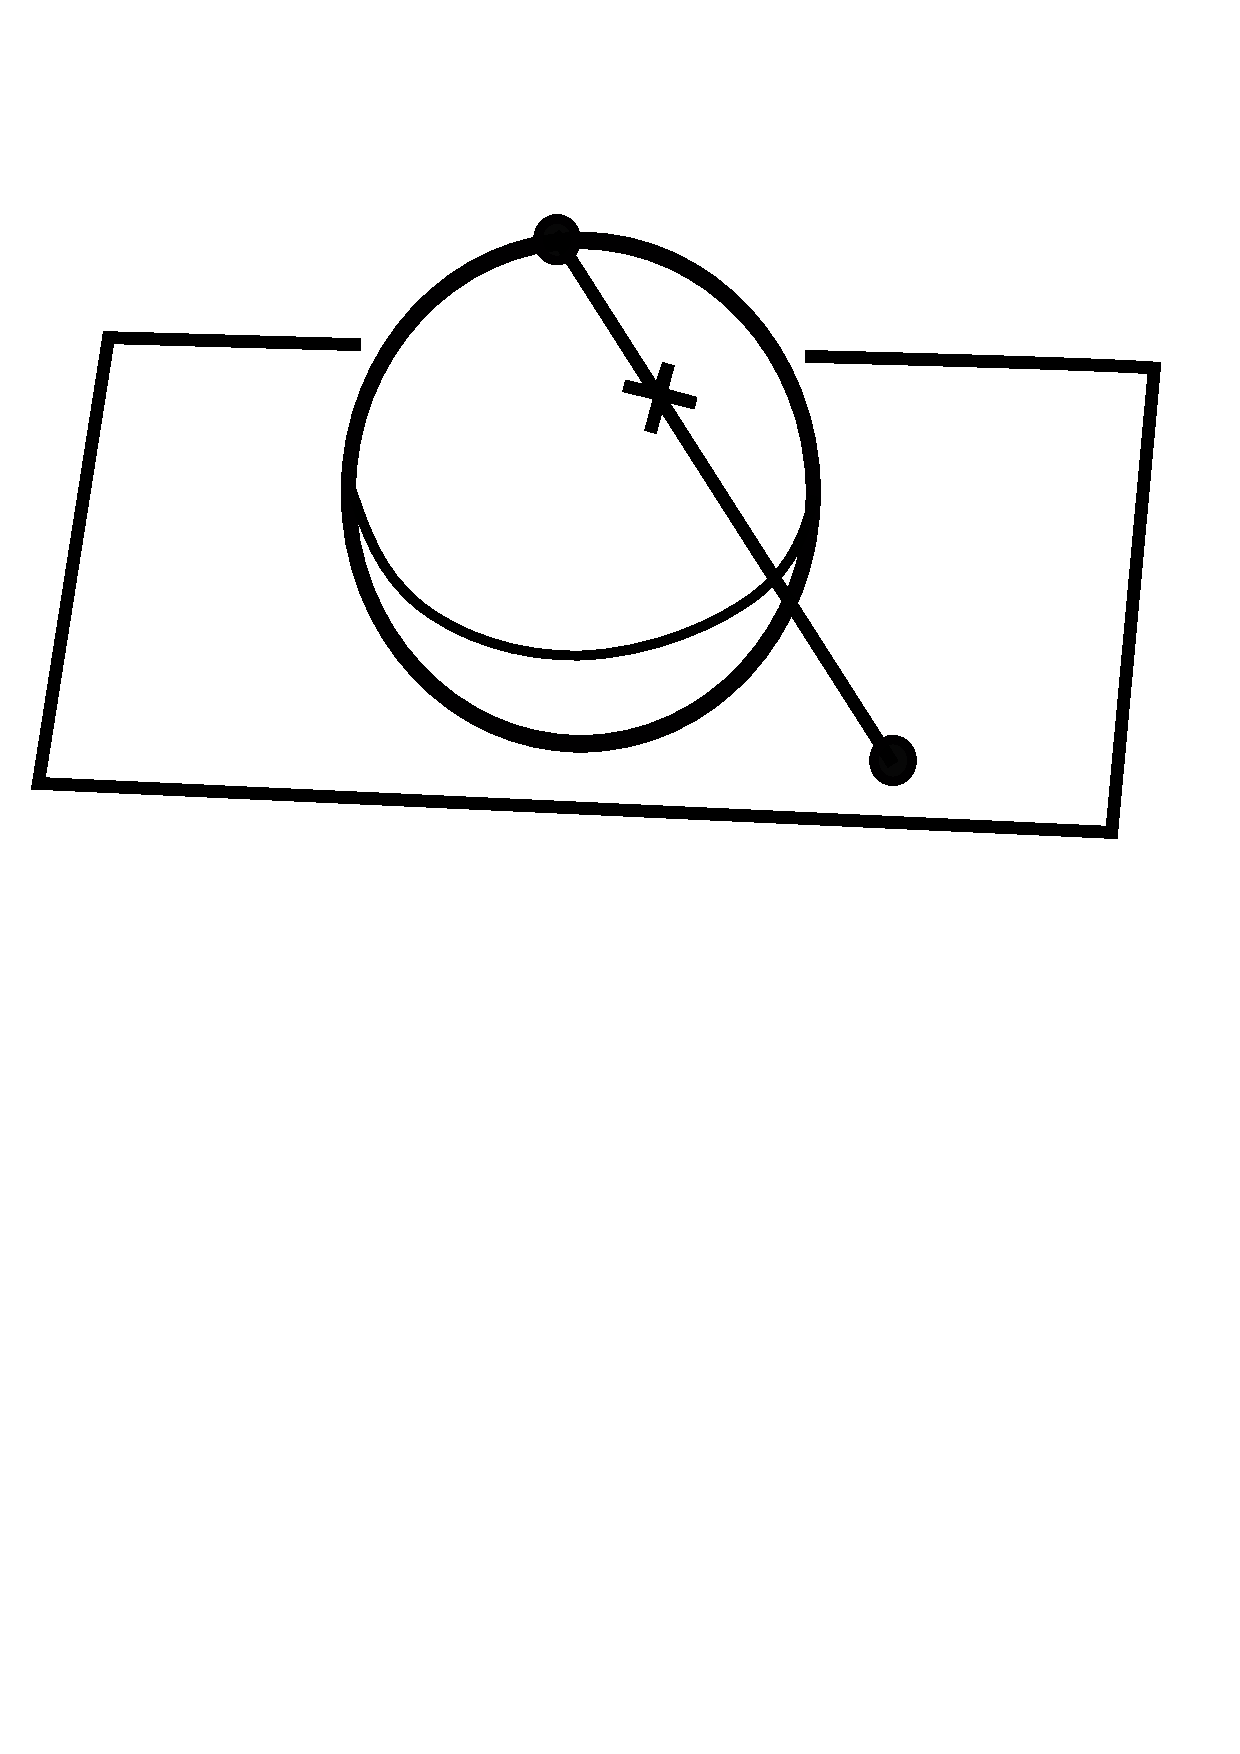
\includegraphics[width=.3\textwidth]{curvature/stereo}
	\caption{A point on the sphere is mapped to a point on the plane by stereographic projection.}
	\label{fig:stereo}
\end{figure}
	
The inverse is given by $p^{-1}:\R^2\to \R^3$

	\begin{equation}\label{eqn:stereo}
		p^{-1}(u,v)=\left(\frac{2u}{u^2+v^2+1},\frac{2v}{u^2+v^2+1},\frac{u^2+v^2-1}{u^2+v^2+1}\right).	
	\end{equation}
To compute the first fundamental form of $p^{-1}(u,v)$ we take the partial derivatives

$$p^{-1}_u=\left(\frac{2v^2-2u^2+2}{(u^2+v^2+1)^2},\frac{-4uv}{(u^2+v^2+1)^2},\frac{4v}{(u^2+v^2+1)^2}\right)$$
and 
$$p^{-1}_v=\left(\frac{-4uv}{(u^2+v^2+1)^2},\frac{2v^2-2u^2+2}{(u^2+v^2+1)^2},\frac{4v}{(u^2+v^2+1)^2}\right).$$
Then, after some algebra,
$$E=p^{-1}_u\cdot p^{-1}_u=\frac{4}{(u^2+v^2+1)^2}$$
$$F=p^{-1}_v\cdot p^{-1}_v=\frac{4}{(u^2+v^2+1)^2}$$
and
$$M=p^{-1}_u\cdot p^{-1}_v=0.$$

We can use the first fundamental form to compute
the  arc length of circles on the sphere parallel to the $xy$ plane with fixed height $z=c$ for $-1<c<1$.
One can compute this length using
the pythagorean theorem. We will see that using stereographic projection
and the first fundamental form we get the same answer.
First, use the map $p$ to map such a circle to the plane.
Using \eqnref{stereo}, our circle on the sphere maps 
to a circle in the plane because
	$$p^{-1}(u,v)=\frac{u^2+v^2-1}{u^2+v^2+1}=c$$
and we can compute the radius in terms of $c$
\begin{equation}\label{eqn:radius}
	u^2+v^2=\frac{1+c}{1-c}=k^2.
\end{equation}
	
In the plane, $u^2+v^2=k^2$ can be parameterized
as $$\gamma(t)=(k\cos(t),k\sin(t))$$ with $0\leq t\leq 2\pi.$
So our curve becomes $p^{-1}\circ \gamma(t)$ on the sphere.
Computing the partial derivatives of $\gamma(t)$ gives
$$\gamma_u'=-k\sin(t)\hspace{1.3cm}  \gamma_v'=k\cos(t).$$
Now we use the first fundamental form

$$\int_{p^{-1}}\gamma ds=\int_{0}^{2\pi} ||(p^{-1}\circ \gamma)'(t)dt=\int_0^{2\pi}\sqrt{E(\gamma_u'(t))^2+2M\gamma_u'\gamma_v'+
F(\gamma_v'(t))^2}dt.$$
Substituting and simplifying using $E=F$ we obtain
$$\int_0^{2\pi}\frac{2k}{k^2+1}dt=\frac{4\pi k}{k^2+1}.$$
Simplifying further using \eqnref{radius}  our arc length is
$$2\pi\sqrt{1-c^2}.$$

\end{example}

\todo{Do we need this? Let $S_1$ and $S_2$ be two surfaces with $\sigma:V\subset S_1\to S_2$ a differentiable map.
At $p\in S_1$ the map $d\sigma_p:T_p(S_1)\to T_{\sigma(p)}(S_2)$ is called the
\EMPH{differential} of $\sigma$ at $p$.}


Stereographic projection has preserves angles and circle.
\todo{define conformal}
We can use conformal maps to obtain a formula
for curvature in terms of the Lapalican?
A few of our applications use the following
formula for Gaussian curvature.

We can always choose a parameterization of a regular surface 
such that the first fundamental form has the form
$E=f(u,v), F(u,v)=0,$ and $G=f(u,v)$ where $f(u,v)>0$


\begin{theorem}[Gaussian Curvature]\label{thm:log-curve}
	Let $f:U\in\R^2\to S$ be an isothermal parameterization of a regular surface.
	The Gaussian curvature, $K,$ of $S$ is 
		\begin{equation}\label{eqn:log-curve}
			K=\frac{-1}{2\lambda}\delta(\log \lambda)
		\end{equation}
\end{theorem}
\begin{proof}
\end{proof}

\subsubsection{Geodesics Curvature}

Shortest paths play an important role in many computational problems.
In a surface, a \EMPH{geodesic} is a curve that is a shortest path
between two points in the surface. 
For example, on $\Sp^2$ great circles are geodesic.
We would like to define the curvature as it would be seen from
someone living on a surface.

Let $U$ be a parameterized chart on a surface $S$ with vector $n(u,v)$ normal
to the surface
and let $\gamma(t)$ be a curve in $U$, with Frenet frame $T,N,B$.
Then $V=n(\gamma(t)\times T$ is in the tangent plane of the surface since
it is perpendicular to $n$. We now have a new orthonormal basis at a point on $\gamma$
namely, $T,V,n$. 
We would like to measure how the rate of change of the tangent vector $T$ with respect to $V$.
The \EMPH{geodesic curvature} is  
\begin{equation} \label{eqn:geodesic}
	k_g=\langle \gamma''(t),V(t)\rangle
\end{equation}
For an alternative equivalent definition see \cite{doc76}.
\todo{non great circle on sphere image}





%%%%%Euler Characteristic%%%%%%%%
\subsection{Triangulations and The Euler Characteristic}

We assume the reader is familiar with the notions
of topological spaces and simplicial complexes.
Most introductory topology texts describe these objects \cite{jm08,munkres}.
The applications we will encounter will refer to triangulated surfaces in $\R^3$
called a \EMPH{mesh}, in one application the surface will contain its interior.
Each triangle in a mesh is isomorphic to a triangle in the plane and the sum
of the interior angles is $\pi$.


We denote the set of vertices, edges and faces in a triangulated surface as 
$V, E$ and $F$ respectively.
Let $\partial(V)$ denote vertices on the boundary of a surface and let $V_{int}$ 
denote vertices that are not on the boundary.
See \figref{triangulated-torus} for an example of a triangulated surface.



The \EMPH{Euler Characteristic} of a surface $\chi$ is the 
the number of vertices minus the number of edges plus  the number of faces, $\chi=|V|-|E|+|F|.$
In higher dimensions, for a triangulated space $X$ the Euler characteristic is 
$\chi(X)=k_0-k_1+k_2-k_3+\ldots$ where $k_n$ is the number of simplices of dimension $n.$
The Euler characteristic is a topological invariant of a space
and does not depend on the choice of triangulation.


Two dimensional spheres $\Sp^2$ and two dimensional disk $D^2$ 
will be used in our applications.
For the sphere, we have $\chi(\Sp^2)=2$ 
several proofs of this can be found on David Eppstein's website \cite{eppstein-proofs}.
For the disk, $\chi(D^2)=1$. The disk can be triangulated by
a single solid triangle with three vertices, three edges and one face.



The \EMPH{genus} of a surface is the maximum number of closed simple
non-intersecting curves that can be drawn in the surface without separating
the surface.
The torus in \figref{triangulated-torus} has genus one.
By the classification of surfaces \cite{munkres}, the Euler characteristic or an orientable surface
is determined by its genus with $\chi=2-2g$.



\begin{figure}[htb]
\centering
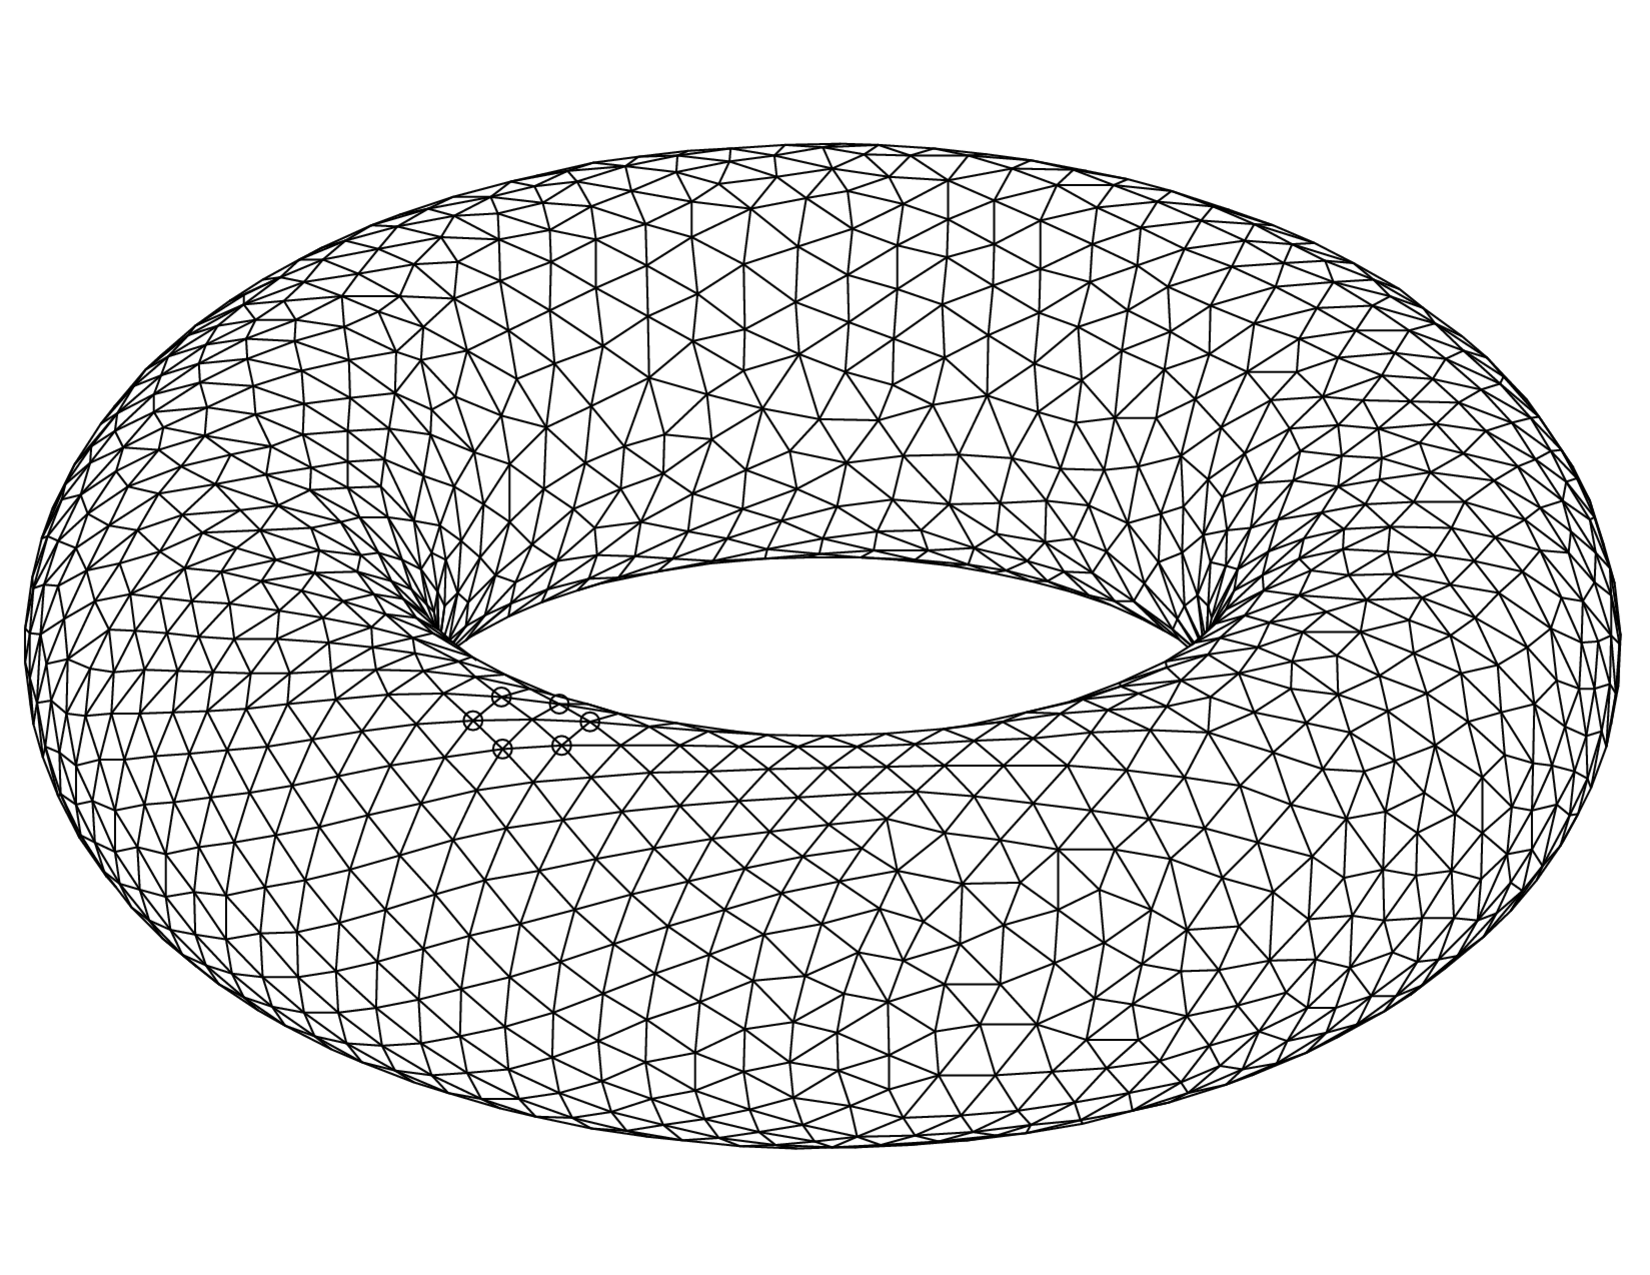
\includegraphics[width=.3\textwidth]{background/Torus-triang}
\caption{A triangulation of the torus. Image from wikipedia.}
\label{fig:triangulated-torus}
\end{figure}

%%%%%Euler Characteristic%%%%%%%%


Using these definitions we can state a continuous version of
the Gauss-Bonnet Theorem for regular surfaces
\begin{theorem}[The Continuous Gauss-Bonnet Theorem] \label{thm:g-b-c}

$$\int_{M} K dA+ \int_{\partial M} k_g ds = 2\pi \chi(M)$$
where $M$ is a regular surface, $K$ is the continuous Gaussian curvature,
 $k_g$ is the continuous geodesic curvature and
$\chi$ is the Euler characteristic.
\end{theorem}

\begin{proof}
	What proof do we want here?
\end{proof}

\subsection{A Discrete Version}
There are several ways to define curvature in the discrete setting \cite{Crane:2013}.
For a piecewise linear curve in $\R^2$, 
if two segments are co-linear, the curvature should be zero.
The curvature should signed, there are two ways we can turn in
the plane.
The exterior angle described above has these properties.
We can express the exterior angle as $\pi$ minus the interior angle.

The one dimensional curves we encounter will be the boundaries
of two dimensional surfaces in $\R^3.$
In a triangulated surface, the interior angle might consist of many triangles.
For a vertex $v$ on the boundary of a surface, 
let $F_v$  denote the set of incident faces and let
$\alpha_f$ denote the angle in face $f$ at $v$.
The \EMPH{discrete geodesic curvature}
of $v$  is
$$k_{g}(v)= \pi-\sum_{f\in F_v}\alpha_f.$$
Notice that if $v$ lies on a straight line, then $\sum_{i}\alpha_f=\pi$
and the curvature is zero as we would expect.
The word geodesic refers to measuring how close
a curve is to being straight with respect to the surface we are on.
This idea can be defined rigorously in the continuous setting \cite{doc76},
in some sense discrete curvature is an oxymoron. 



Next, we consider a vertex in a discrete surface that is not on the boundary.
Again, we require that a vertex on a flat surface has zero curvature.
One definition of Gaussian curvature is the following

\begin{definition}[Discrete Gaussian curvature]\label{def:discrete-curvature-vertex}

The discrete \EMPH{Gaussian curvature} at a vertex $v$ is the area on the unit 
sphere bounded by a spherical polygon whose vertices are the unit normals of 
the faces around $v$.

\end{definition}

If a vertex is on a flat surface, then the unit normals are all pointed
in the same direction and the  Gaussian curvature is zero.

\begin{figure}[htb]
\centering
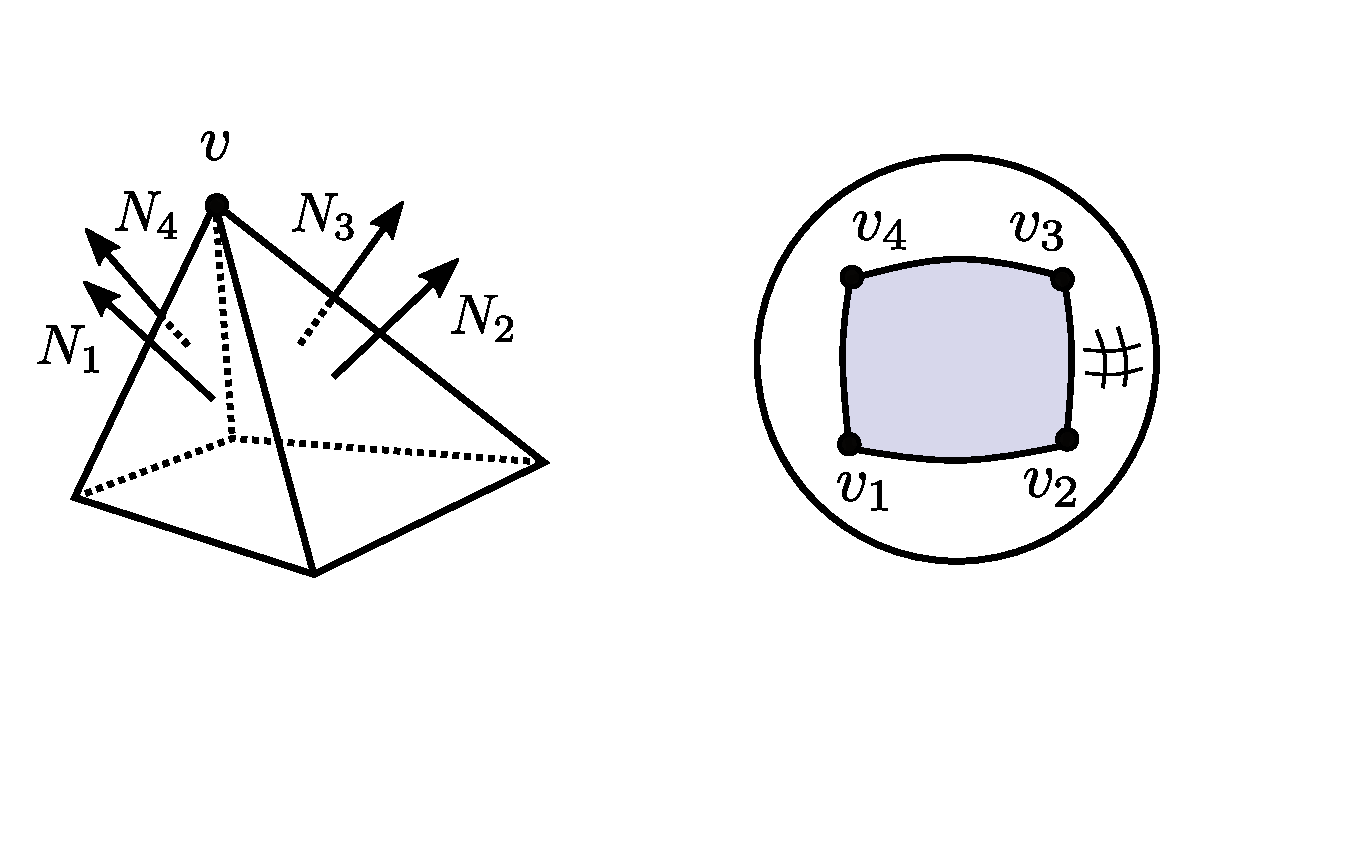
\includegraphics[width=.5\textwidth]{curvature/discrete-curvature}
\caption{Consider the vertex $v$ on the left. The curvature of $v$
is the area on the sphere shown on the right. We rotated the sphere
in order to see the entire polygon.}
\label{fig:discrete-curvature}
\end{figure}


\eqnref{sphere-area} gives a formula for computing the curvature at a vertex, provided
we know the interior angles of the polygon on the sphere.
The interior angles of the polygon $\beta_i$ on the sphere are supplementary to
the angle $\alpha_i$ incident to $v$ in the surface

\begin{equation} \label{eqn:switcheroo}
\beta=\pi-\alpha.
\end{equation}
To see this, notice that the edge between two faces
is perpendicular to the normal vectors of the faces.
vectors is perpendicular to both normal vectors. 

two normal vectors will intersect the edge between the vectors 
at right angles. 

We can then consider the triangles show in
 \figref{switcheroo}.


\begin{figure}[htb]
\centering
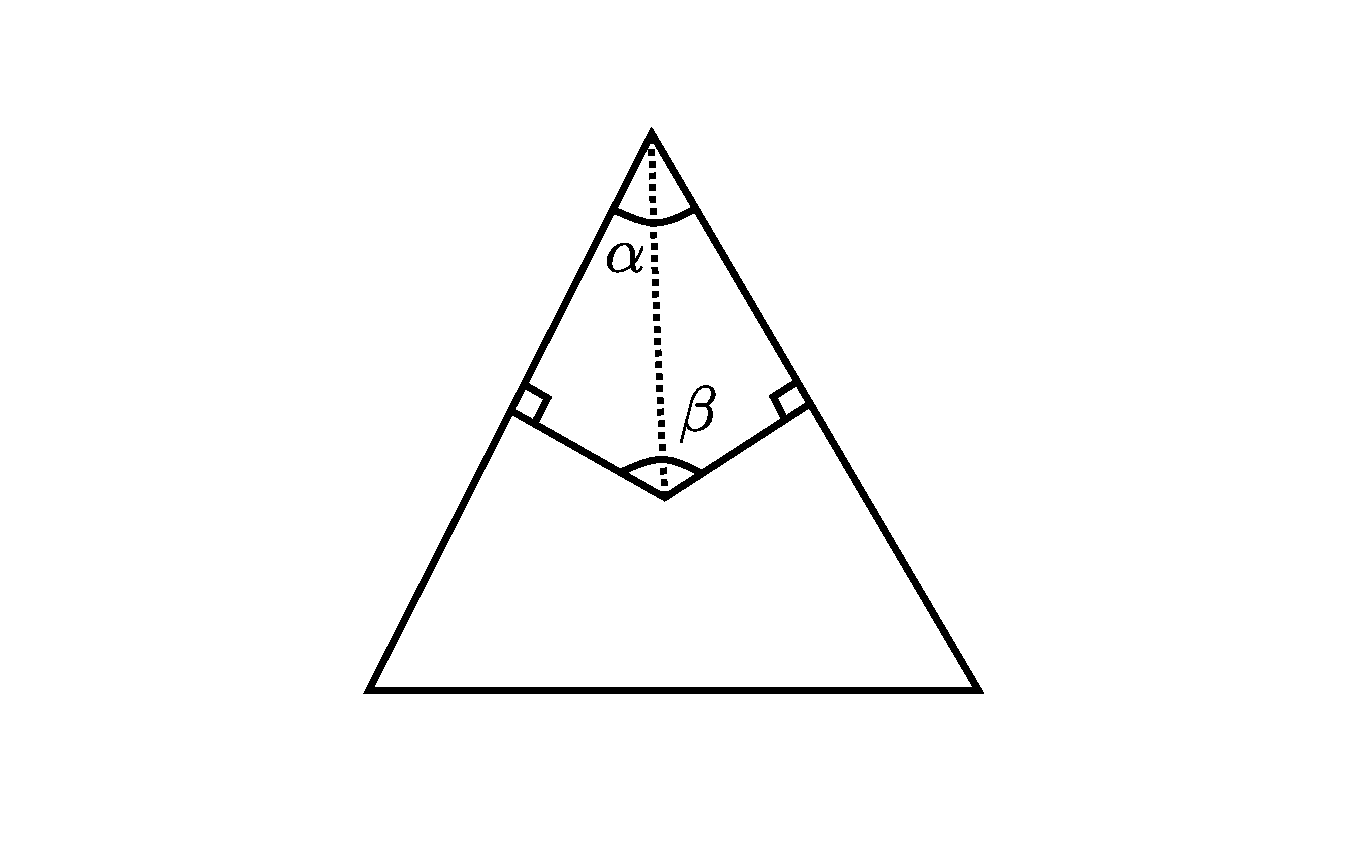
\includegraphics[width=.3\textwidth]{background/switch-angles}
\caption{The relationship between the angles incident to a vertex and
the interior angles of the area polygon on the sphere.}
\label{fig:switcheroo}
\end{figure}



This gives a convenient formula for computing the curvature at an interior vertex.
The \EMPH{angle defect} at a vertex $d(v)$ is the difference between $2\pi$ and
the sum of the incident angles.  Let $F_v$ denote the faces containing $v$  
and let $\alpha_f$  denote the interior  angle of face $f$ at $v$, then
\begin{equation} \label{eqn:defect}
d(v):=2\pi -\sum_{f\in F_v}\alpha_f.
\end{equation}
Since $\beta_i=\pi-\alpha_i$, we have the Gaussian curvature at $v$
is 
$$K(v)=2\pi -n\pi+\sum_{i}^n \beta_i=2\pi-n\pi +\sum_{i}^n (\pi-\alpha_i) =2\pi-\sum_i^n\alpha_i=d(v)$$
 and the
 angle defect is equal to the discrete curvature in \defref{discrete-curvature-vertex}.







Putting all of these variables together gives

\begin{theorem}[The Discrete Gauss-Bonnet Theorem] \label{thm:g-b-d}

$$\sum_{v\in V_{int}} K(v) + \sum_{v\in V_{\partial S}} k_g(v) = 2\pi \chi(S)$$
where $S$ is a triangulation, $K(v)$ is the discrete Gaussian curvature
of a vertex, $k_g(g)$ is the discrete geodesic curvature and
$\chi$ is the Euler characteristic.
\end{theorem}

The  Gauss-Bonnet theorem is  telling us, if we add up curvature
at each vertex the sum will be $2\pi$ times to Euler characteristic.
If we can compute the curvature at every vertex then we can use the theorem
to learn global topological information.
Conversely, if we know the Euler characteristic we can learn about the curvature
at individual points.

